% Add photos or diagrams of the observatory
\section{Motivation}

\begin{frame}
\frametitle{Motivation}

\begin{itemize}
	\item In Chile, the astronomy has become one of the scientific fields with a surprising growth rate in the last years.
	\item There are more than a dozen astronomical facilities in our country, for example:
		\begin{enumerate}
			\addtolength{\itemindent}{1cm}
			\item Atacama Large Millimeter/submillimeter Array (ALMA)
			\item Very Large Telescope (VLT)
			\item And soon the European Extremely Large Telescope (E-ELT)
		\end{enumerate}
\end{itemize}

\begin{center}
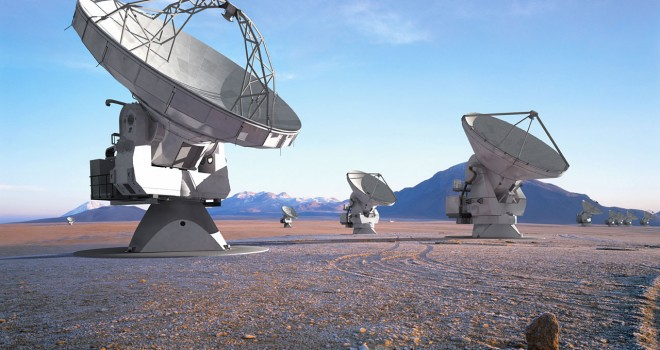
\includegraphics[height=0.3\textheight]{img/alma}
\end{center}


\end{frame}



\begin{frame}
\frametitle{Motivation}

\begin{itemize}
	\item One of the conditions established in our country, is that the 10\% of the observation
		time belongs to the Chilean astronomical community
	\item \textbf{Motivation}: it's necessary to develop an astroinformatic platform for the data administration
		and intelligent analysis.
\end{itemize}

\begin{center}
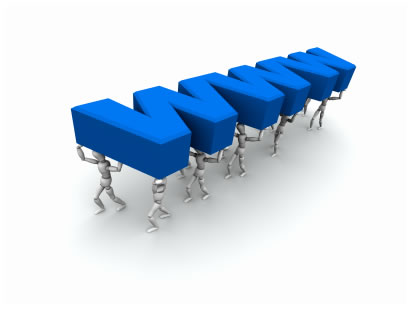
\includegraphics[height=0.3\textheight]{img/platform}
\end{center}


\end{frame}
